\section{Experiments and Results}\label{chap:experiments_results}
In this section, we present the experimental validation of our SVM implementations. We start with a synthetic linearly separable dataset to compare the primal and dual formulations, followed by experiments with non-linear data using various kernels, and finally evaluate performance on the real-world Breast Cancer Wisconsin dataset.

\subsection{Experimental Setup}
The SVM algorithms were implemented as described in Section~\ref{chap:problem}, with both primal and dual formulations. 
For optimization, we used subgradient descent with Barzilai-Borwein step sizing for the primal problem and a projected gradient ascent algorithm for the dual problem.

\subsection{Linear Separable Data}
We first generate a linearly separable synthetic dataset with $n = 52$ points in 2D using \texttt{make\_toy\_data} function to create data with a clear margin between the two classes.

\subsubsection{Primal SVM}
We trained the Primal SVM with $C=1.0$ using subgradient descent for 10,000 iterations with a learning rate of 0.001 and Barzilai-Borwein steps. 
Figure~\ref{fig:primal_svm} shows the decision boundary, margins, and support vectors identified by the model.

\begin{figure}[H]
    \centering
    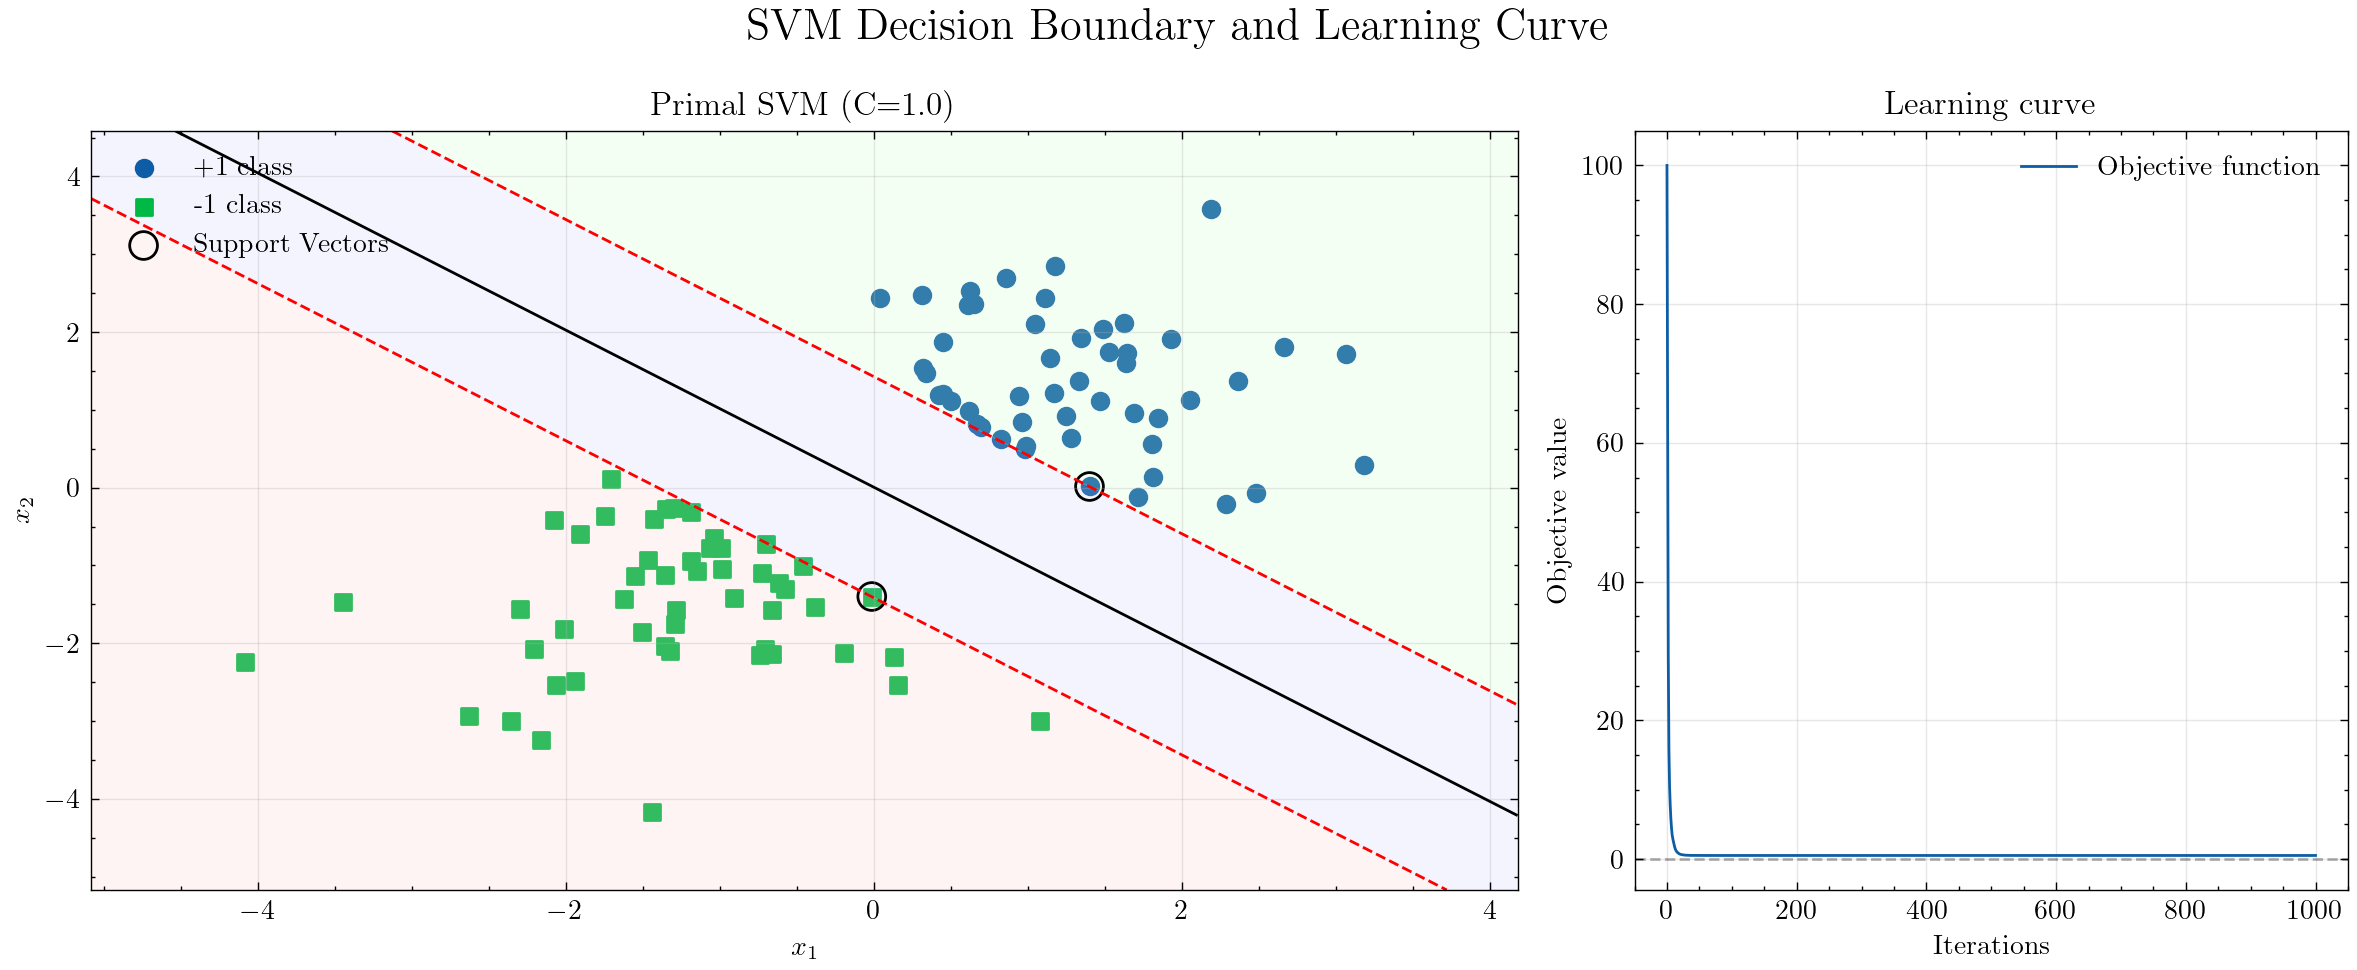
\includegraphics[width=0.90\textwidth]{figures/primal_svm.png}
    \caption{Primal SVM with linear kernel ($C=1.0$). The solid line represents the decision boundary, and the dashed lines represent the margins. Support vectors are highlighted with green circles.}
    \label{fig:primal_svm}
\end{figure}

The primal formulation achieved 100\% accuracy on the training data. The algorithm correctly identified two support vectors (one from each class), which lie exactly on the margin boundaries. The weight vector $\mathbf{w}$ converged to approximately $[0.7069, 0.7073]$ with a bias term $b = -0.001$, resulting in a maximum margin hyperplane.

\subsubsection{Dual SVM with Linear Kernel}
We trained the Dual SVM with the same $C=1.0$ parameter using a linear kernel. The dual formulation also achieved 100\% accuracy and identified the same support vectors as the primal approach. Figure~\ref{fig:dual_svm} shows the resulting decision boundary.

\begin{figure}[H]
    \centering
    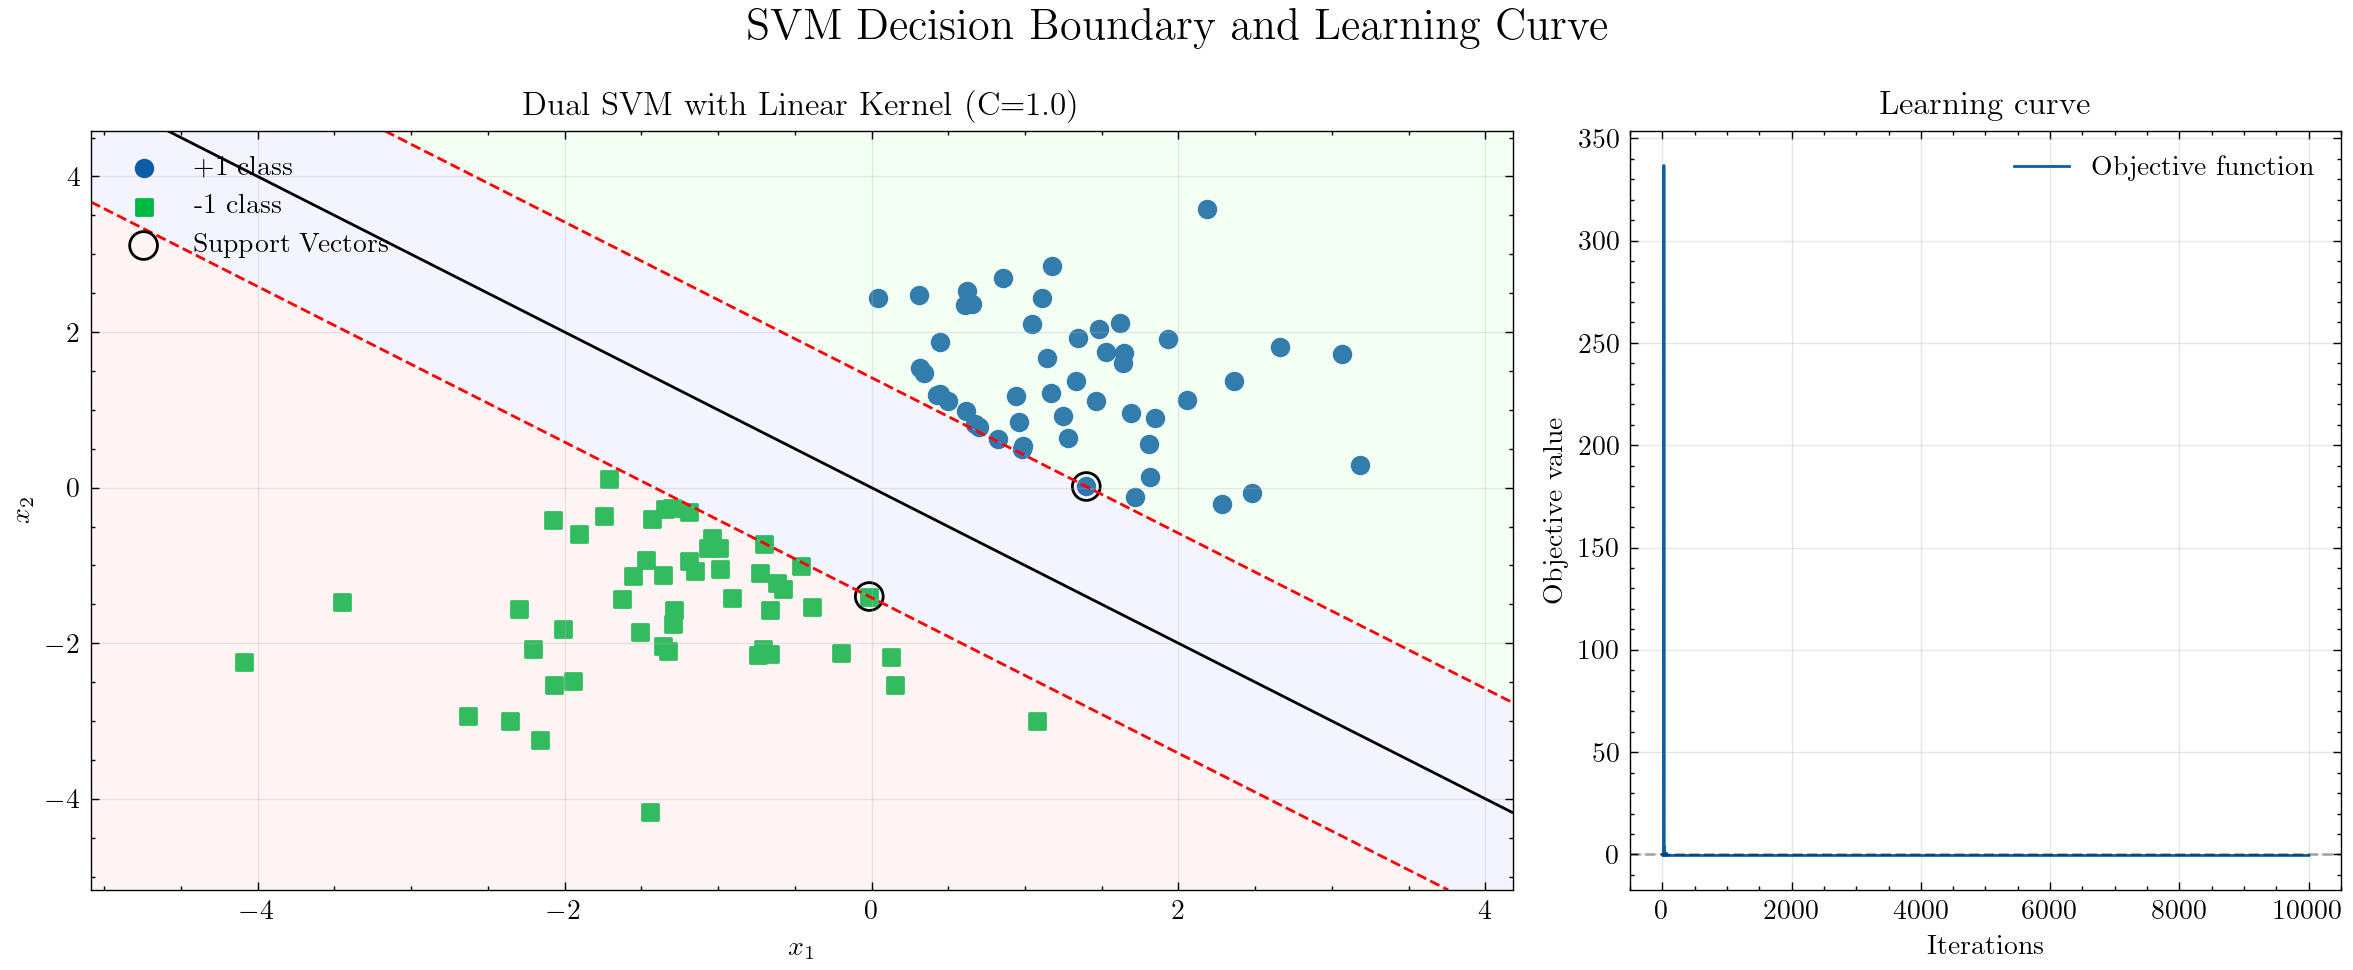
\includegraphics[width=0.90\textwidth]{figures/dual_svm.png}
    \caption{Dual SVM with linear kernel ($C=1.0$). The decision boundary and margins are nearly identical to those found by the primal formulation.}
    \label{fig:dual_svm}
\end{figure}

When we recovered the weight vector from the dual solution using $\mathbf{w} = \sum_{i=1}^{n} \alpha_i y_i \mathbf{x}_i$, we obtained $\mathbf{w} \approx [0.7071, 0.7071]$, which is just the normalized primal solution. 
This confirms the theoretical equivalence of the primal and dual formulations for linear separable data.

\subsection{Effect of Regularization Parameter}
To understand the impact of the regularization parameter $C$, we trained the primal SVM with three different values: $C = \{0.1, 1.0, 10.0\}$. 
Figure~\ref{fig:c_values} shows how the decision boundaries and margins change with different $C$ values.

\begin{figure}[H]
    \centering
    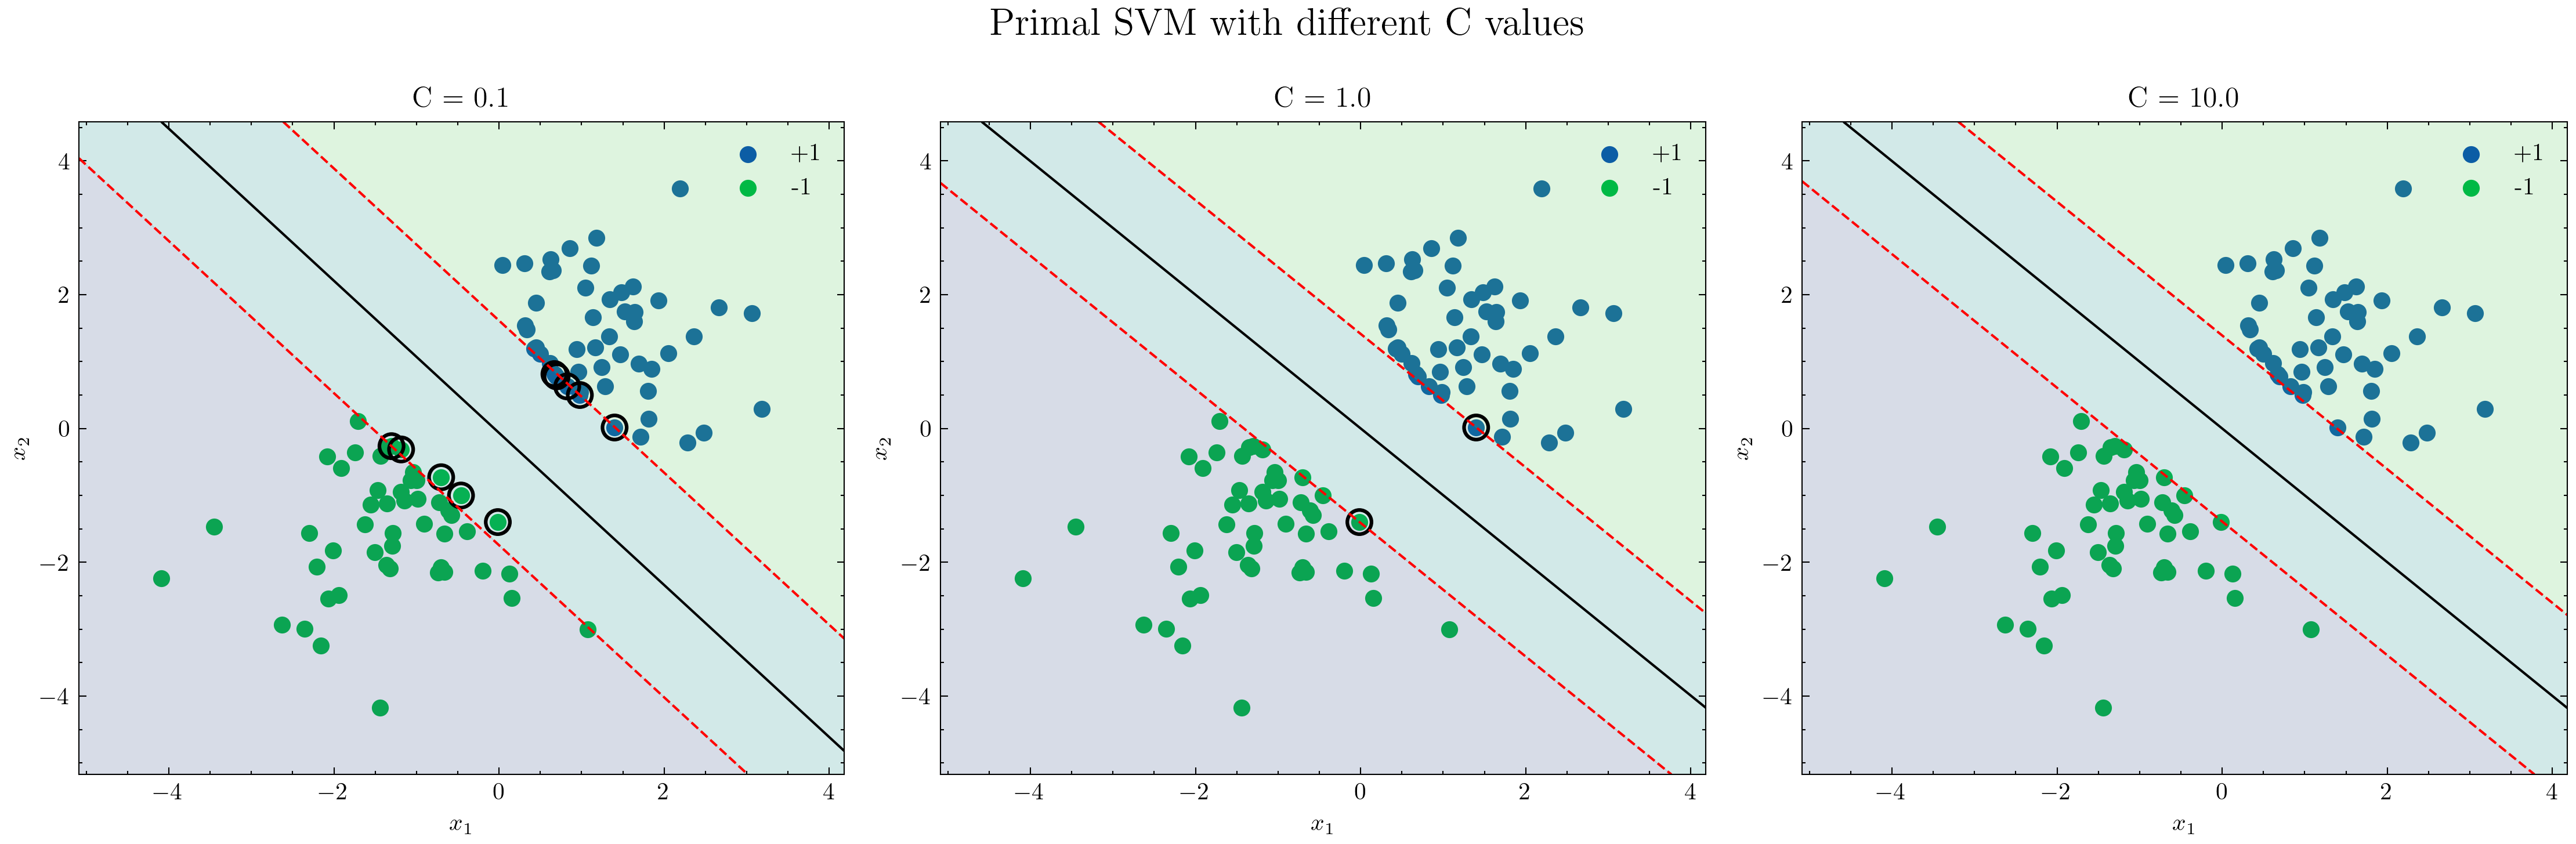
\includegraphics[width=0.95\textwidth]{figures/primal_svm_c_values.png}
    \caption{Comparison of different $C$ values in Primal SVM. Lower $C$ values (left) result in wider margins but may allow more training errors, while higher $C$ values (right) enforce stricter classification at the cost of narrower margins.}
    \label{fig:c_values}
\end{figure}

We observe that:
\begin{itemize}
    \item With $C = 0.1$ (low regularization), the model prioritizes a wider margin at the potential cost of misclassifications.
    \item With $C = 1.0$ (balanced), we achieve a good trade-off between margin width and classification accuracy.
    \item With $C = 10.0$ (high regularization), the model focuses more on reducing training errors, potentially leading to narrower margins and possible overfitting.
\end{itemize}

\subsection{Non-linear Data with Different Kernels}
We next evaluate our dual SVM implementation on non-linearly separable data using different kernels. Figure~\ref{fig:kernels} shows the performance of four different kernels on a synthetic dataset with circular decision boundaries.

\begin{figure}[H]
    \centering
    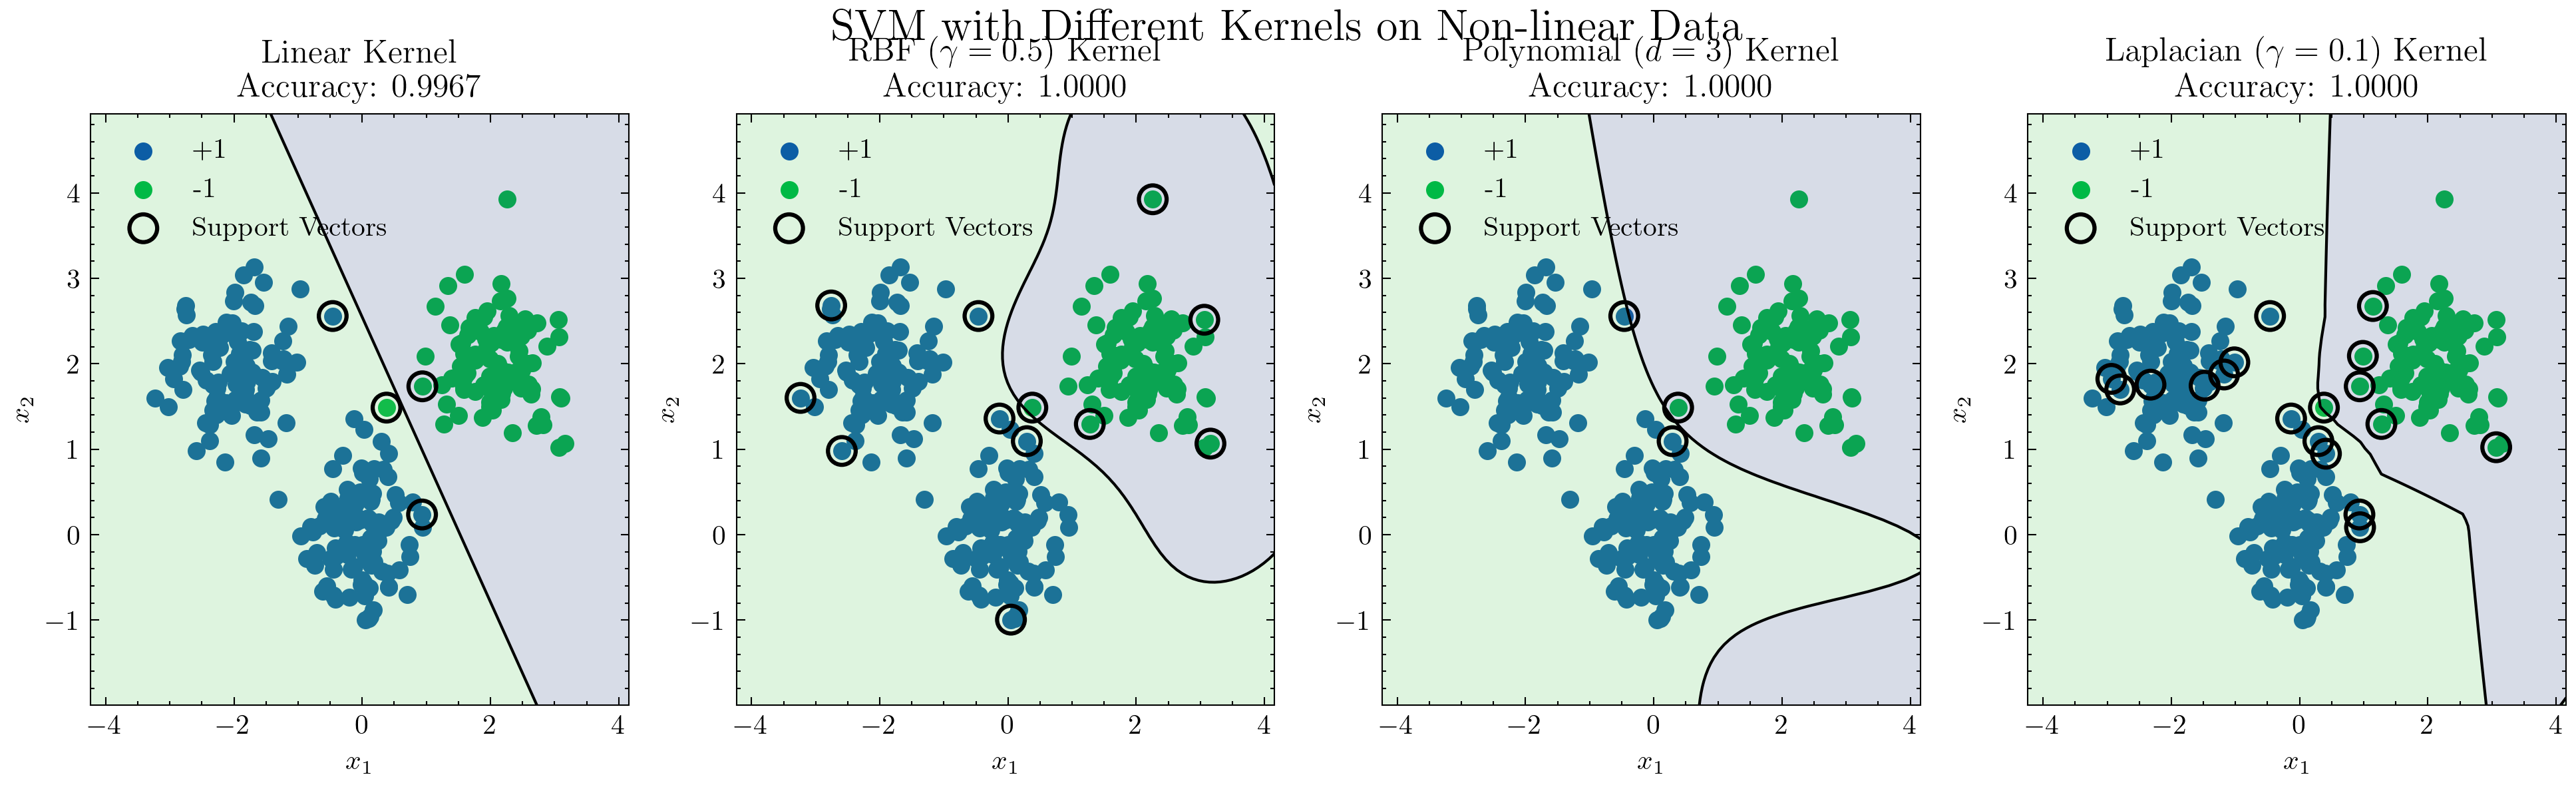
\includegraphics[width=0.95\textwidth]{figures/svm_kernels_comparison.png}
    \caption{Comparison of different kernels on non-linear data. From left to right: Linear, RBF, Polynomial, and Laplacian kernels.}
    \label{fig:kernels}
\end{figure}

As expected, the linear kernel performs poorly on this non-linear dataset, achieving only around 50\% accuracy. The RBF kernel with $\gamma=0.5$ perfectly captures the circular decision boundary with 100\% accuracy. The polynomial kernel (degree 3) also performs well but creates a more complex decision boundary. The Laplacian kernel ($\gamma=0.1$) also achieves 100\% accuracy with a smooth decision boundary.

This experiment demonstrates the power of the kernel trick in handling non-linear classification tasks without explicitly mapping features into a higher-dimensional space.

\subsection{Breast Cancer Wisconsin Dataset}
Finally, we applied our SVM implementation to the Breast Cancer Wisconsin dataset, which contains 30 features computed from digitized images of fine needle aspirates (FNA) of breast mass, with binary labels indicating benign or malignant tumors.

\subsubsection{Model Selection}
We evaluated multiple kernel types (Linear, RBF, Polynomial, Laplacian) with different $C$ values (0.1, 1.0, 10.0) on this dataset. Table~\ref{tab:cancer_results} shows a subset of the results.

\begin{table}[H]
    \centering
    \begin{tabular}{lccc}
        \toprule
        \textbf{Kernel} & \textbf{C} & \textbf{Train Accuracy} & \textbf{Test Accuracy} \\
        \midrule
        Linear & 0.1 & 0.9824 & 0.9825 \\
        Linear & 1.0 & 0.9868 & 0.9561 \\
        Linear & 10.0 & 0.5077 & 0.5175 \\
        RBF ($\gamma=0.01$) & 0.1 & 0.9516 & 0.9649 \\
        RBF ($\gamma=0.01$) & 1.0 & 0.9758 & 0.9649 \\
        RBF ($\gamma=0.01$) & 10.0 & 0.9912 & 0.9825 \\
        Polynomial (d=2) & 1.0 & 0.7780 & 0.7719 \\
        Laplacian ($\gamma=0.1$) & 1.0 & 0.9934 & 0.9649 \\
        \bottomrule
    \end{tabular}
    \caption{Performance of different SVM configurations on the Breast Cancer Wisconsin dataset.}
    \label{tab:cancer_results}
\end{table}

The RBF kernel with $C=10.0$ achieved the best test accuracy of 98.25\%. Interestingly, the linear kernel with $C=0.1$ performed nearly as well, suggesting that the data might be largely linearly separable in the original feature space. The dramatic drop in performance for the linear kernel with $C=10.0$ indicates possible numerical issues or instability with high regularization values.

\subsubsection{PCA Visualization}
To visualize the decision boundaries in this high-dimensional dataset, we applied Principal Component Analysis (PCA) to reduce the data to 2 dimensions, then trained an RBF kernel SVM on this reduced representation. Figure~\ref{fig:cancer_pca} shows the result.
\begin{figure}[H]
    \centering
    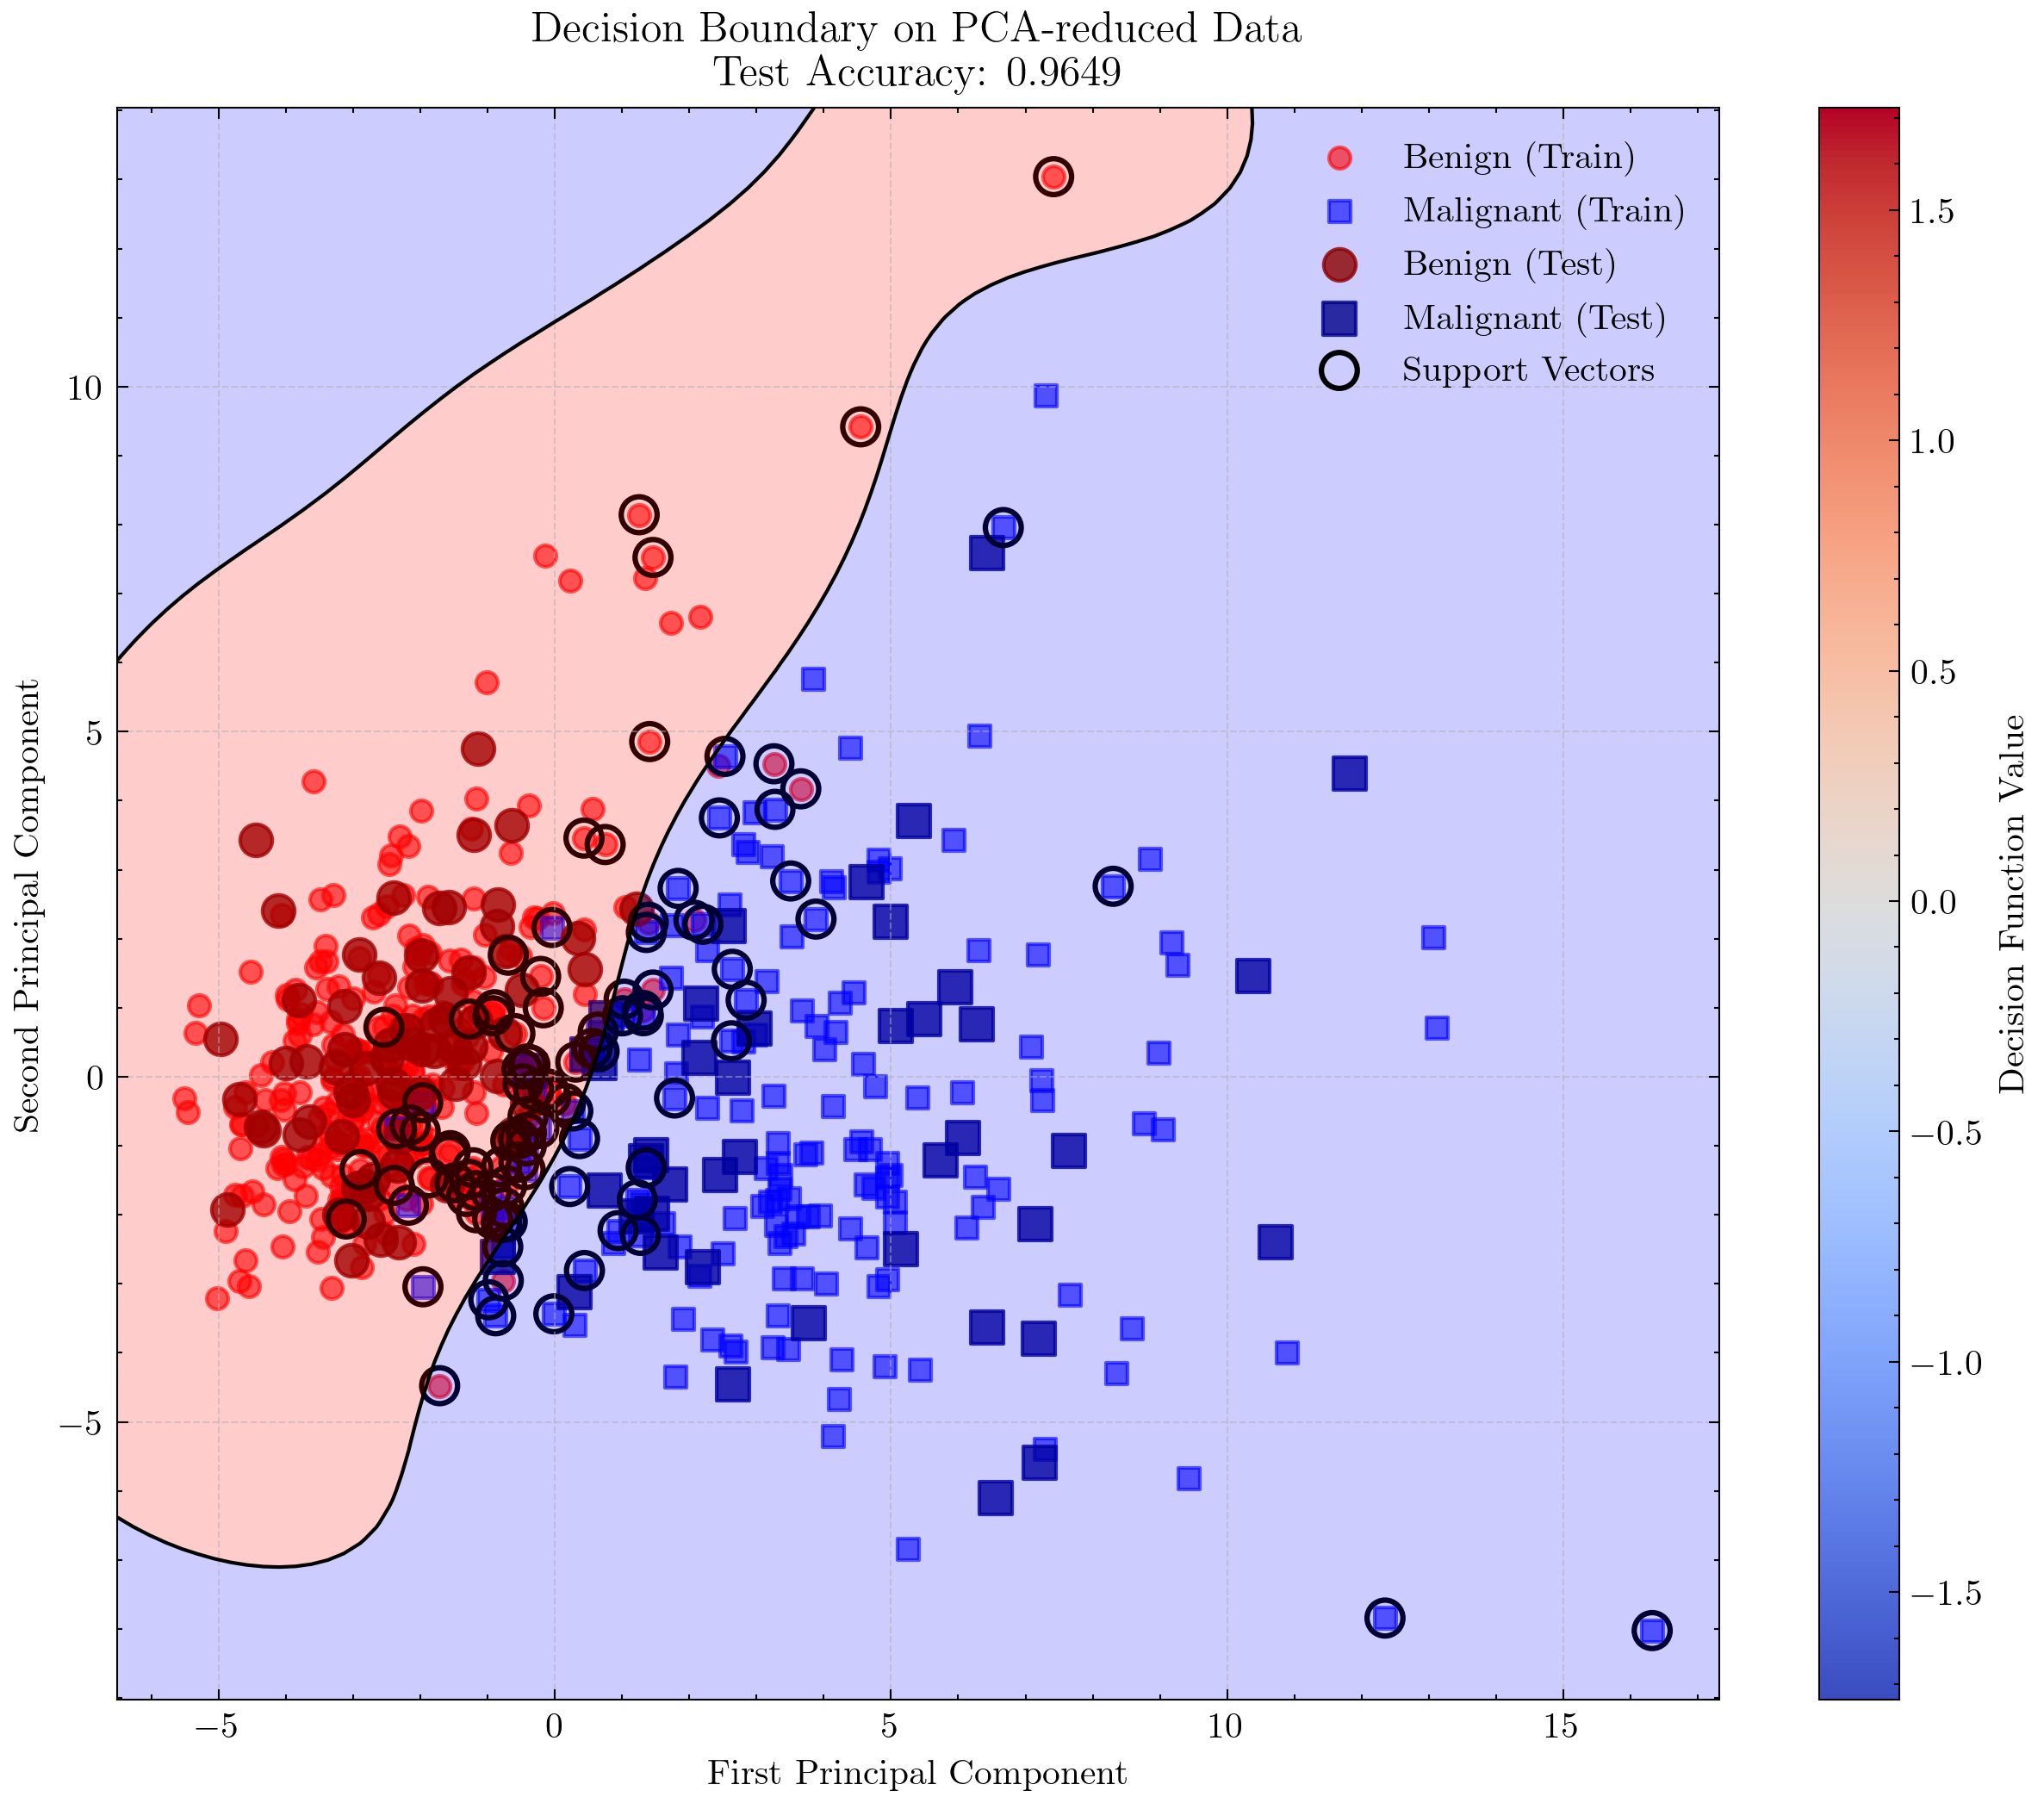
\includegraphics[width=0.7\textwidth]{figures/breast_cancer_pca.png}
    \caption{Decision boundary visualization of the Breast Cancer dataset after PCA reduction. Red points represent benign tumors, blue points represent malignant tumors, and black circles indicate support vectors.}
    \label{fig:cancer_pca}
\end{figure}
From the PCA analysis, we found that the first two principal components explain approximately 63\% of the variance in the data. The most important features contributing to the first component include mean concavity, mean concave points, and worst concave points, suggesting that these characteristics are crucial for distinguishing between benign and malignant tumors.

\subsection{Discussion}
Our experiments demonstrate several key insights about SVMs:

\begin{enumerate}
    \item For linear separable data, both primal and dual formulations achieve identical results, confirming their theoretical equivalence.
    
    \item The regularization parameter $C$ significantly affects the trade-off between margin width and training error. Selecting an appropriate $C$ value is crucial for good generalization.
    
    \item Non-linear kernels dramatically improve performance on datasets where classes are not linearly separable. The choice of kernel and its parameters can significantly impact the model's decision boundary.
    
    \item On real-world data like the Breast Cancer dataset, SVMs can achieve high accuracy, especially when using appropriate kernels. The RBF kernel generally performed best across our experiments, but the linear kernel was surprisingly effective on the cancer dataset.
    
    \item While the algorithms achieve high accuracy, they required careful tuning of optimization parameters (learning rates, tolerance thresholds, maximum iterations) to ensure convergence.
\end{enumerate}

These results highlight the versatility and effectiveness of SVMs for classification tasks, especially when combined with appropriate kernel functions for non-linear problems.

